%!TEX root = ../scivis_lbaakman_bvanloon.tex

\chapter{Color Mapping} % (fold)
\label{cha:color_mapping}

Color mapping is widely used for the visualization of scalar data. This is done by coloring the shapes based the scalar value that is visualized. \Cref{s:colormapping:introduction} discusses several color maps, and some things that should be considered when implementing a color map. The next section discusses how we have implemented our color maps. Finally, \cref{s:colormapping:results} shows the results of applying color maps to our data set.  

\section{Introduction}
\label{s:colormapping:introduction}
%!TEX root = ../scivis_lbaakman_bvanloon.tex

\begin{figure}
	\centering
	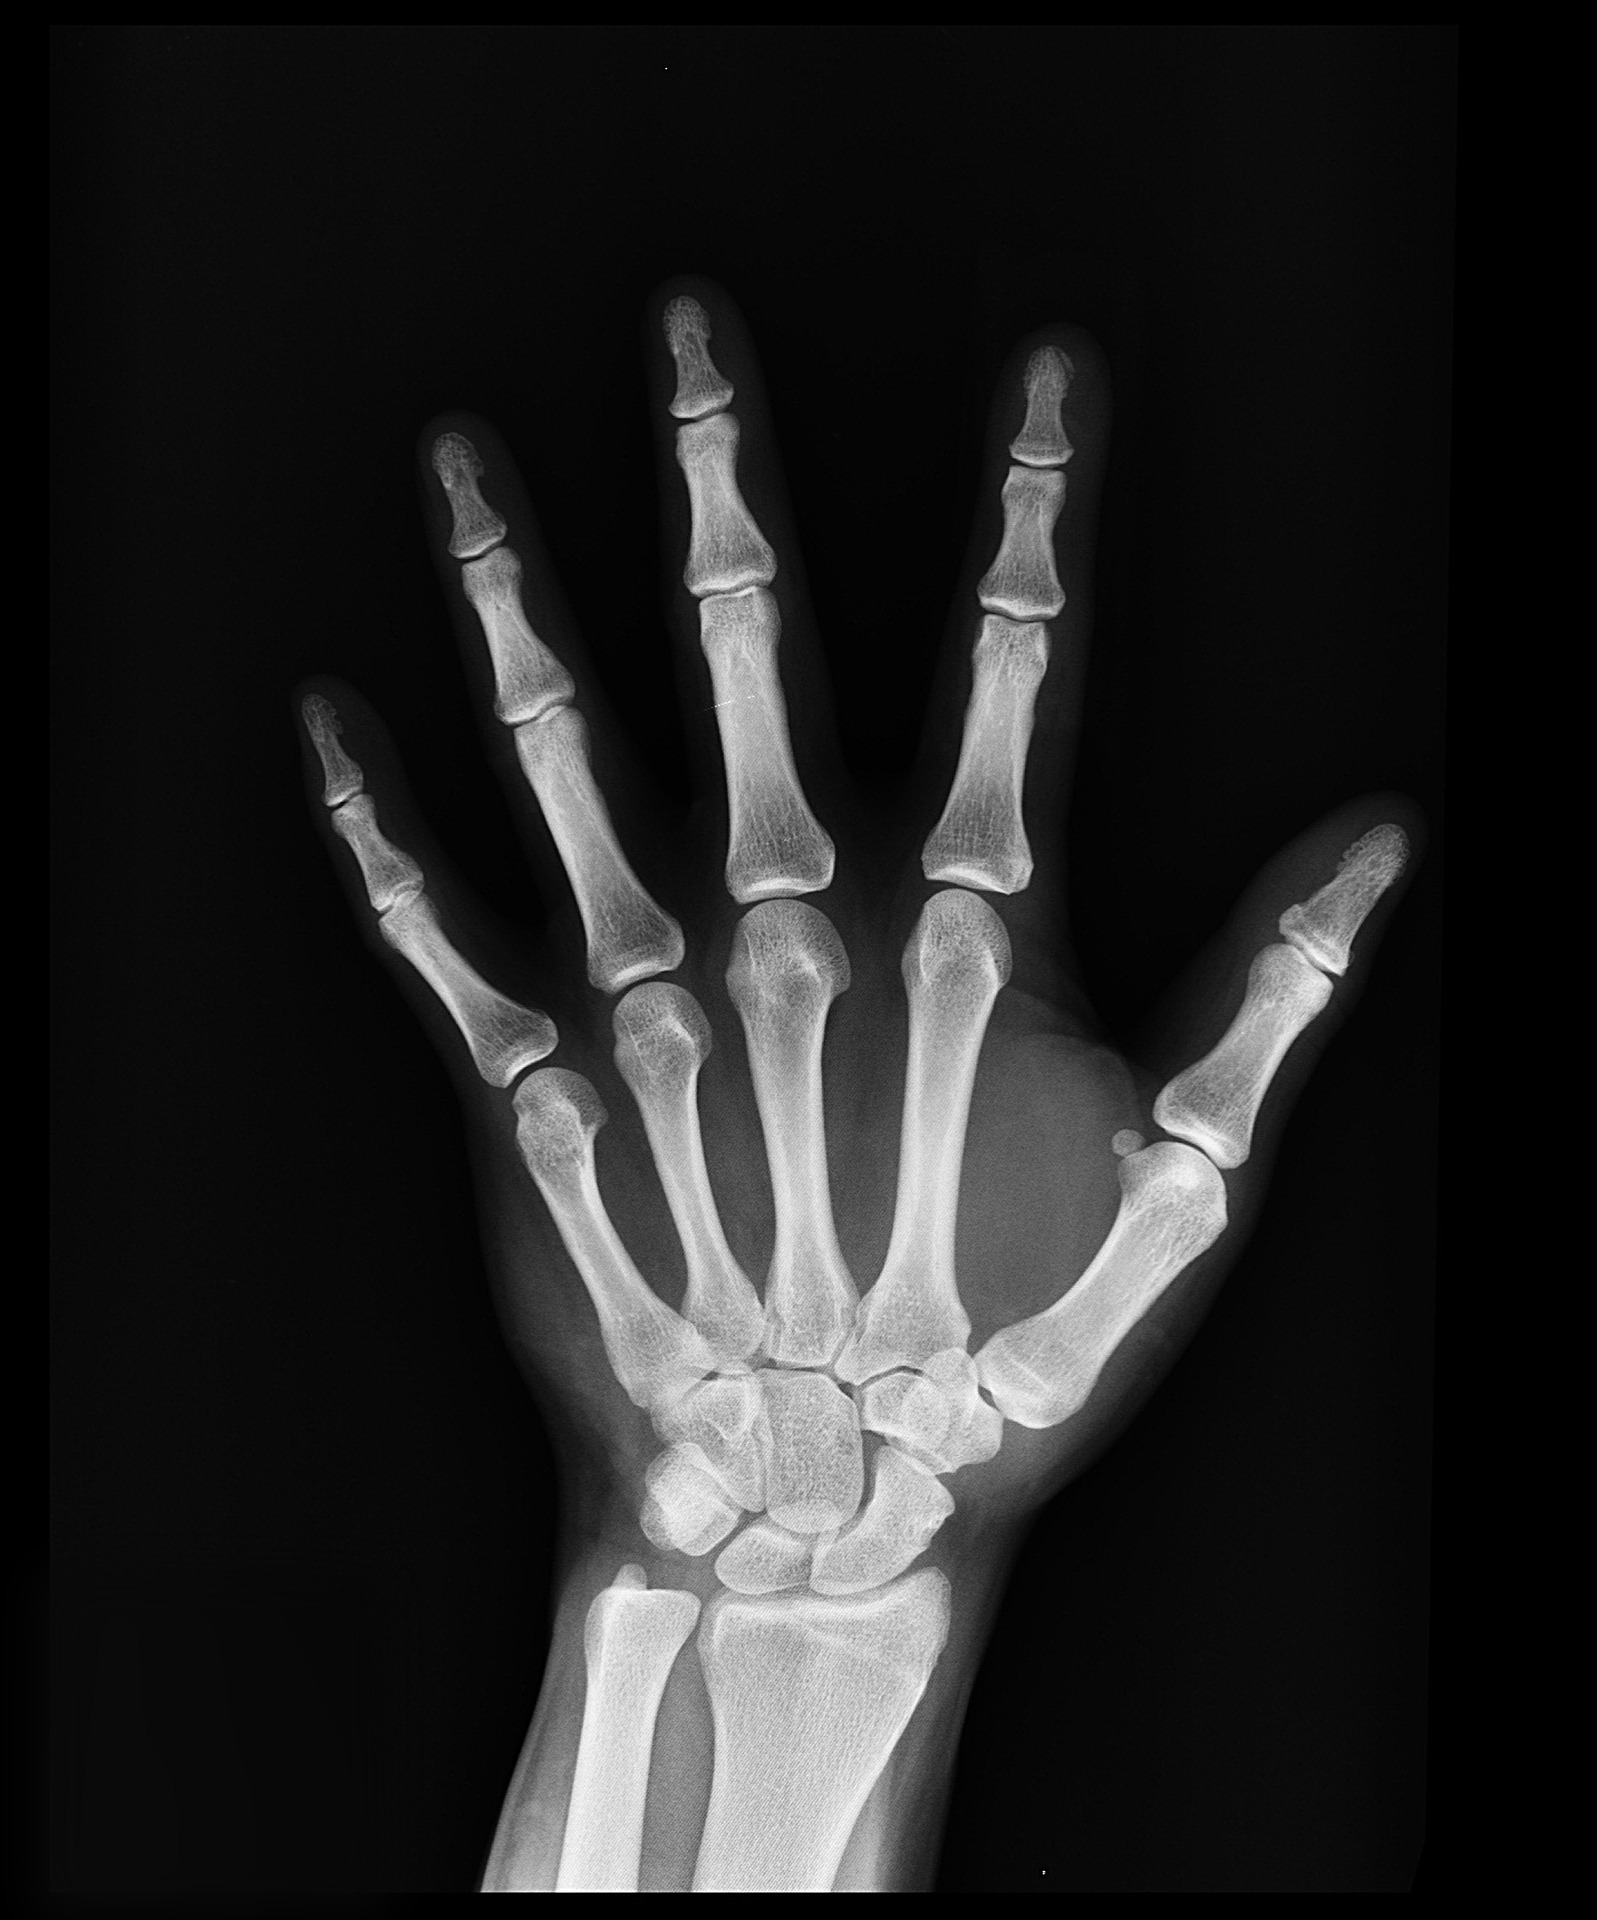
\includegraphics[width=0.5\textwidth, height=0.2\textheight, keepaspectratio]{colormapping/img/x-ray.jpg}
	\caption{An example of the use of a color map, image from \cite{xray}.}
	\label{fig:colormapping:xray}
\end{figure}

\Cref{fig:colormapping:xray} shows a well known example of the use of a color map. In this image lighter colors are used to indicate areas where the density of the X-rayed object are high, whereas darker colors represent areas of low density. X-rays use gray scale color maps, that is it maps the density values of the object to colors ranging from black to white. \Cref{s:colormapping:introduction} discusses the gray scale color map extensively and introduces other color maps. In \cref{ss:colormaps:parameterization} the parameterization of these color maps is introduced. \Cref{ss:colormaps:applying} discusses techniques that can be used to map the scalar data to the color maps. In the final section, \cref{ss:colormaps:variables}, the application of the color maps to the scalar variables in our application is discussed. 

\subsection{Different Color Maps}
\label{ss:colormaps:differentmaps}

\begin{figure}
	\centering
	\begin{subfigure}{\textwidth}
		\centering
		\includegraphics[width=\textwidth]{./img/_}
		\caption{Rainbow color map, $\varDX = 0.8$.}
		\label{fig:colormapping:intro:differntColorMaps:rainbow}
	\end{subfigure}
	\begin{subfigure}{\textwidth}
		\centering
		\missingfigure{ColorMap to be generated}
		% \includegraphics[width=\textwidth]{./img/_}
		\caption{Gray scale color map.}
		\label{fig:colormapping:intro:differntColorMaps:grayscale}
	\end{subfigure}	
	\begin{subfigure}{\textwidth}
		\centering
		% \includegraphics[width=\textwidth]{./img/_}
		\missingfigure{ColorMap to be determined}
		\caption{Undetermined color map.}
		\label{fig:colormapping:intro:differntColorMaps:ofChoice}
	\end{subfigure}		
	\caption{A visualization of different color maps: \subref{fig:colormapping:intro:differntColorMaps:rainbow} rainbow, \subref{fig:colormapping:intro:differntColorMaps:grayscale} gray scale, and \subref{fig:colormapping:intro:differntColorMaps:ofChoice} unknown color map.}
	\label{fig:colormapping:introduction}
\end{figure}

	% Rainbow ColorMap
	\todo[inline]{Discuss Rainbow colormap: advantages, disadvantages, influence of dx}		

	% GrayScale ColorMap
	\todo[inline]{Discuss GrayScale color map: advantages, disadvantages}

	% ColorMap of Choice
	\todo[inline]{Discuss Chosen color map: advantages, disadvantages, why this one}
	

	

\subsection{Parameterization of Color Maps}
\label{ss:colormaps:parameterization}
	\todo[inline]{Number of colors, disadvantages/advantages when to use?}
	\todo[inline]{Change hue, disadvantages/advantages when to use?}
	\todo[inline]{Change saturation, disadvantages/advantages when to use?}

\subsection{Applying Color Maps}
\label{ss:colormaps:applying}
	\todo[inline]{Discuss clamping}
	\todo[inline]{Discuss scaling}

\subsection{Variables that the Color Maps are Applied to}
\label{ss:colormaps:variables}
	\todo[inline]{Discuss fluid density, what is it? suitable for colormapping? Which colormap?}
	\todo[inline]{Discuss fluid velocity magnitude what is it? suitable for colormapping? Which colormap?}
	\todo[inline]{Discuss force field magnitude what is it? suitable for colormapping? Which colormap?}


\section{Method}
\label{s:colormapping:method}
%!TEX root = ../../scivis_lbaakman_bvanloon.tex
\section{Method}
\label{s:streamsurfaces:method}
This section explains how one can define a stream surface given a seed curve \seedCurve, with $n$ vertices, $\seedCurveVertex{0}, \cdots ,\seedCurveVertex{n}$ and $T$ two-dimensional vector fields, $\vectorFieldDiscTime{}{0}, \cdots, \vectorFieldDiscTime{}{T}$,  that represent the different states of some vector field as a function of time.


In \cref{s:streamsurface:method:time} we explain how we compute a three dimensional streamline in a number of consecutive two dimensional datasets. \Cref{s:streamsurface:method:seedCurve} explain how we compute the seed points given the seed curve \seedCurve. \Cref{s:streamsurface:method:surface} discusses how we define a stream surface from a set of streamlines. 

\subsection{Time as the Third Dimension}
\label{s:streamsurface:method:time}
We start the streamline at seed point \seedPoint{0} in the two-dimensional vector field \vectorFieldDiscTime{}{T}, \ie the oldest vector field that we have. We then compute the next vertex of the two-dimensional streamline in the vector field \vectorFieldDiscTime{}{T} with seed point \seedPoint{0}. We refer to this two-dimensional position as \seedPoint{1}. This position is used as the seed point of a two-dimensional streamline of one edge in the vector field \vectorFieldDiscTime{}{T - 1}. The other vertex of that edge is referred to as \seedPoint{2}, and is used as the seed point in \vectorFieldDiscTime{}{T - 2}. This process is repeated until we have reached \vectorFieldDiscTime{}{0}. 

The points $\seedPoint{0}, \cdots, \seedPoint{T}$ define the three dimensional stream line. The \textit{z}-coordinate of these points is computed in such a way that the points are spread uniformly in \textit{z} over some predefined range for \textit{z}.


The streamline is thus computed according to the process described in \cref{cha:streamlines}, with one change: there is no lower bound for the magnitude, \ie $\magnitudeMin = \infty$.

\subsection{From a Seed Curve to Seed Points}
\label{s:streamsurface:method:seedCurve}
The seed curve is a polyline, each of the line segments of this polyline is split into \resolution segments. The higher \resolution is the better the final stream surface is. 

\subsection{Building the Surface}
\label{s:streamsurface:method:surface}
The final step of defining a stream surface is the determination of a surface from a set of streamlines, \streamLineIdx{0}, \streamLineIdx{N}. The line segments of the stream lines are have all approximately the same length, as the distance between \seedPoint{i} and \seedPoint{i + 1} is equal for every segment in every stream line and the difference in \textit{z}-coordinates of consecutive stream line vertices is also equal. We then define the stream surface by connecting vertex \seedPoint{i} of stream line \streamLineIdx{j} with \seedPoint{i} of stream line \streamLineIdx{j + 1}, for $j < N$. If stream line \streamLineIdx{j} has a vertex \seedPoint{i}, but \streamLineIdx{j + 1} is shorter and does not have a \seedPoint{i}, we connect \seedPoint{i} of \streamLineIdx{j} to the last vertex of \streamLineIdx{j + 1}.


The resulting connections define a collection of quads that could define a surface. However the thus defined surface would happily move though some obstacle that is encountered by the flow of the vector field. To avoid this we do not connect two neighboring vertices of streamlines if the distance between them is greater than \divergenceCriterion. 


\section{Results}
\label{s:colormapping:results}
%!TEX root = ../../scivis_lbaakman_bvanloon.tex
\section{Results}
\label{s:streamsurfaces:results}
This section presents and discusses several visualizations of the evolution of a two-dimensional vector field as a function of time with stream surfaces. All visualizations in this section will show the fluid velocity, and will be colored according to the fluid velocity magnitude with a color map that is not clamped. The older simulation states are shown near the bottom of the images, more recent states are shown near the top of the images.

\begin{figure}
	\centering
	\begin{subfigure}{0.7\textwidth}
		\centering
		\assusScreenshot[height=0.27\textheight, keepaspectratio=true]{./img/streamsurfaces/vertices}
		\caption{Vertices}
		\label{fig:streamsurfaces:differentmethods:vertices}
	\end{subfigure}
	\begin{subfigure}{0.7\textwidth}
		\centering
		\assusScreenshot[height=0.27\textheight, keepaspectratio=true]{./img/streamsurfaces/lines}
		\caption{Stream Lines}
		\label{fig:streamsurfaces:differentmethods:lines}
	\end{subfigure}	
	\begin{subfigure}{0.7\textwidth}
		\centering
		\assusScreenshot[height=0.27\textheight, keepaspectratio=true]{./img/streamsurfaces/surface}
		\caption{Stream Surface}
		\label{fig:streamsurfaces:differentmethods:surface}
	\end{subfigure}		
	\caption{Visualization of the change of a two-dimensional vector field, \velocity, as function of time with \subref{fig:streamsurfaces:differentmethods:vertices} the vertices of the stream lines, \subref{fig:streamsurfaces:differentmethods:lines} the stream lines and \subref{fig:streamsurfaces:differentmethods:surface} the stream surface. %
	\resolution = 10, \numStates = 200, \divergenceCriterion = 200.0.}
	\label{fig:streamsurfaces:differentmethods}
\end{figure}

We support three different ways of visualizing a stream surface. Firstly one can use the vertices of the streamlines as shown in \cref{fig:streamsurfaces:differentmethods:vertices}. Alternatively one can visualize the streamlines as in \cref{fig:streamsurfaces:differentmethods:lines}, or the surface defined by these lines as in \cref{fig:streamsurfaces:differentmethods:surface}. 

\Cref{fig:streamsurfaces:differentmethods:surface} clearly illustrates one issues of our stream surfaces, firstly the edges of the computational domain are not reached gracefully. It is possible that this is caused by the fact that our streamlines end at their last vertex before the end of the computational domain, instead of on the edge of the domain.

It should be noted that the resolution of seed lines used for the visualizations in \cref{fig:streamsurfaces:differentmethods} was chosen quite low, to emphasize the difference between the lines and the vertices.

The straight streamlines at the bottom of these figures, \ie in the oldest simulation states, are caused by lack of user input at the beginning. In that case, all vectors are \vec{0}, consequently $\seedPoint{i} = \seedPoint{i + 1}$, which results in a line segment whose vertices only differ in their \textit{z}-values.

\Cref{fig:streamsurfaces:differentResolution} presents three visualizations of the same data set with three different resolutions. This figures clearly illustrates the importance of choosing a resolution that is sensible for the data, in this case a resolution of five is clearly too low, \resolution = 50, seems sufficient. If resolution is set to 100 the stream lines are so close together that they nearly form a surface. 

\begin{figure}
	\centering
	\begin{subfigure}[b]{0.3\textwidth}
		\centering
		\threeDScreenshot{./img/streamsurfaces/r5}
		\caption{\resolution = 5}
		\label{fig:streamsurfaces:differentResolution:r5}
	\end{subfigure}
	\begin{subfigure}[b]{0.3\textwidth}
		\centering
		\threeDScreenshot{./img/streamsurfaces/r50}
		\caption{\resolution = 50}
		\label{fig:streamsurfaces:differentResolution:r50}
	\end{subfigure} 
	\begin{subfigure}[b]{0.3\textwidth}
		\centering
		\threeDScreenshot{./img/streamsurfaces/r100}
		\caption{\resolution = 100}
		\label{fig:streamsurfaces:differentResolution:r100}
	\end{subfigure} 
	\caption{Visualization of the change of a two-dimensional vector field, \velocity, as function of time with different resolutions. %
	\numStates = 200}
	\label{fig:streamsurfaces:differentResolution}
\end{figure}

The influence of the \divergenceCriterion is illustrated in \cref{fig:streamsurfaces:differentDivergenceCriterion}. To more clearly show the divergence both the stream lines and the stream surfaces are shown. Since the length of the stream lines are not influenced by \divergenceCriterion they are always visible independent of the divergence of the vector field.

The influence of the \divergenceCriterion can be seen in the size of the triangle that is placed between the flow that moves to the left and the flow to the right. The higher the divergence criterion the longer the two flows are connected. If \divergenceCriterion = 3 the stream splits quite early, whereas for \divergenceCriterion = 200 the streams stay together until \rfrac{1}{3} of the y-axis. The influence of the divergence criterion is also illustrated in the upper left corner of these images. 

\begin{figure}
	\centering
	\begin{subfigure}[b]{0.3\textwidth}
		\centering
		\threeDScreenshot{./img/streamsurfaces/d3}
		\caption{\resolution = 3}
		\label{fig:streamsurfaces:differentDivergenceCriterion:r3}
	\end{subfigure}
	\begin{subfigure}[b]{0.3\textwidth}
		\centering
		\threeDScreenshot{./img/streamsurfaces/d30}
		\caption{\resolution = 30}
		\label{fig:streamsurfaces:differentDivergenceCriterion:r30}
	\end{subfigure} 
	\begin{subfigure}[b]{0.3\textwidth}
		\centering
		\threeDScreenshot{./img/streamsurfaces/d200}
		\caption{\resolution = 200}
		\label{fig:streamsurfaces:differentDivergenceCriterion:r200}
	\end{subfigure} 
	\caption{Visualization of the change of a two-dimensional vector field, \velocity, as function of time with different divergence criteria. %
	\resolution = 100, \numStates = 200.}
	\label{fig:streamsurfaces:differentDivergenceCriterion}
\end{figure}

\Cref{fig:streamsurfaces:differentVectorFields} shows the stream lines of two different vector fields, namely the fluid velocity field and the force field. \Cref{fig:streamsurfaces:differentVectorFields:force} clearly illustrates that the added forces decays quite quickly. This visualization also shows that the stream lines are straight lines as long as the vector fields don't change as a function of time at the position of the seed point.

\begin{figure}
	\centering
	\begin{subfigure}[b]{0.3\textwidth}
		\centering
		\threeDScreenshot{./img/streamsurfaces/fluidVelocity}
		\caption{\velocity}
		\label{fig:streamsurfaces:differentVectorFields:velocity}
	\end{subfigure}
	\begin{subfigure}[b]{0.3\textwidth}
		\centering
		\threeDScreenshot{./img/streamsurfaces/force}
		\caption{\force}
		\label{fig:streamsurfaces:differentVectorFields:force}
	\end{subfigure}  
	\caption{Visualization of the change of \subref{fig:streamsurfaces:differentVectorFields:velocity} fluid velocity field and \subref{fig:streamsurfaces:differentVectorFields:force} the force field as a function of time. 
	%
	\resolution = 100, \numStates = 200}
	\label{fig:streamsurfaces:differentVectorFields}
\end{figure}

% chapter color_mapping (end)